\title{LCCR: An R Package for Inference on Latent Class Models for Capture-Recapture Data with Covariates}
\author{by Francesco Bartolucci and Antonio Forcina}

\maketitle

\begin{abstract}
A detailed description of the R package LCCR for the analysis of capture-recapture data relating to a closed population is provided.
The data that can be analyzed consist of the full capture history for each sample unit and may possibly include individual covariates.
The package allows the specification and estimation of latent class models in which the distribution of the capture history conditional on the latent class and covariates follows either a log-linear model in which bivariate interactions are allowed, or a logit model for the conditional probability of capture at each occasion given the previous capture history.
Alternatively, the conditional distribution of each capture occasion can be formulated by a logit model that may account for the effect of previous capture occasions.
Apart from the conditional distribution of the capture history, the covariates can also affect the distribution of the class weights.
Estimation is based on the unconditional maximum likelihood method, suitably extended to account for the presence of covariates by including unit-specific weights, which are commonly used in empirical likelihood methods.
The package also allows simulation of capture-recapture data from a specified model and the computation of the profile confidence interval for the population size.
For illustration, we use a data set about meningitis cases in an Italian region.
\end{abstract}

\section{Introduction}

In the statistical literature on capture-recapture data relating to closed populations, see \cite{BohningBook} for a recent overview, several models are now available, which represent a development of traditional models such as those illustrated in \cite{otis1978statistical}.
Here we focus on the typical case in which, for each unit captured at least once, the full capture history is available.
In this case, the most recent model formulations can address both observed heterogeneity, accounted for by individual covariates, and unobserved heterogeneity, using random effects or latent variables having a continuous or discrete distribution.
Moreover, maximum likelihood estimation may be formulated in two different ways; see \cite{Sanathanan} for a fundamental contribution in this regard.
The simplest method is based on maximizing the conditional likelihood function of the observed data given that sample units have been captured at least once.
This function depends on the model parameters only, which are estimated prior to the population size.
In contrast, the unconditional maximum likelihood (UML) method is based on a target function which is jointly maximized with respect to the population size and model parameters.

In this paper, we focus on a class of models that may address both observed and unobserved heterogeneity, by the inclusion of individual covariates and latent variables having a discrete distribution, and which are described in \cite{bartolucci2024estimating}; this class of models is closely related to the one proposed in \cite{Bart2006} and \cite{bartolucci2007class}.
In particular, we describe the R package \CRANpkg{LCCR} \citep{bart:pkg:2021} that contains functions to formulate and estimate these models.
Estimation is based on the UML method described in \cite{bartolucci2024estimating} that takes inspiration from the formulation based on empirical likelihood \citep{owen2001empirical}, developed by \cite{Liu2017}.
The functions in package \CRANpkg{LCCR} may also be used to simulate data from an assumed model and to obtain a profile confidence interval for the population size, which has interesting properties with respect to standard confidence intervals based on the standard error for this parameter.

In R, other packages are available to deal with capture-recapture data.
Here we mention two among the most popular packages which are available in CRAN and are related to the present package \CRANpkg{LCCR}.
Package \CRANpkg{Rcapture} \citep{baillargeon2007rcapture} provides functions to fit log-linear models for capture-recapture data for closed and open populations, together with tools for preliminary analysis of these data based on descriptive statistics and for model selection and diagnostics.
For closed populations, in particular, the models considered may be specified in different ways to also include behavioral and heterogeneity effects \citep[see also][]{rivest2007applications}, while parameter estimation is based on a conditional maximum likelihood method.
Inference on the population size is also based on the profile likelihood method of \cite{cormack1992interval}.
Another R package that may be used to fit capture-recapture models for closed populations is \pkg{BBRecapture}.
The models considered in the package allow for accounting for behavioral effects in a flexible way; see also \cite{FegaTa2016}.
The inference on these models is based on a Bayesian approach under a set of prior distributions on the parameters, although the package also contains functions for UML estimation.
A related package is \CRANpkg{LCMCR} \citep{manrique-vallier2023} that, by a Markov chain Monte Carlo algorithm, fits a Bayesian non-parametric latent class model for capture-recapture data that does not require specifying the number of classes because it relies on a Dirichlet process, as described in \cite{manrique2016bayesian}.
It is worth noting that, differently from the previous packages, the \CRANpkg{LCCR} package described here allows for individual covariates conditionally on the latent class, apart from permitting the formulation of models with a variety of effects of the type conceptualized by \cite{otis1978statistical}.

The remainder of the paper is organized as follows.
In the next section, we provide an overview of the statistical approach in terms of model assumptions and inferential methods, summarizing some concepts introduced in \cite{bartolucci2024estimating}.
Then, we describe a set of preliminary functions of package \CRANpkg{LCCR} to formulate models, simulate data from the assumed model, and manipulate the available data.
A further section is devoted to the main R functions to estimate model parameters and the population size, also by a profile confidence interval.
The paper concludes with an example based on Italian meningitis data and a brief summary.

\section{Approach overview}
%
Let $J$ denote the number of capture occasions generating configurations denoted by $\bm{r}=(r_1,\ldots,r_J)'$, with $r_j=0,1$, $j\in\mathcal{J}$, where $\mathcal{J}=\{1,\ldots,J\}$.
The set of all possible capture configurations $\bm{r}$ apart from $\bm{0}$ is denoted by $\mathcal{R}$, where in general $\bm{0}$ denotes a column vector of zeros of a suitable dimension; when this set includes the $\bm{0}$ configuration, it is denoted by $\tilde{\mathcal{R}}$.
In the present framework, the units captured at least once, whose number is denoted by $n$, may be collected in $I$ strata with each stratum $i\in\mathcal{I}$, $\mathcal{I}=\{1,\ldots,I\}$, having a corresponding vector of $c$ covariates $\bm{w}_i$.
We also consider the possible presence of vectors of covariates $\bm{x}_{i,j}$, of dimension $d$, which are also specific to the capture occasion.
The observed capture-recapture configurations are represented by the column vectors $\bm{y}_i$ having $2^J-1$ elements $y_{i,\bm{r}}$, $\bm{r}\in\mathcal{R}$, corresponding to the frequency of the capture configuration $\bm{r}$ in stratum $i$.
The sum of these frequencies is denoted by $n_i$, with all the $n_i$ collected in the vector $\bm{n}$.
Note that, with individual data, each vector $\bm{y}_i$ has only one element equal to 1 and all other elements equal to 0, so that $n_i=1$ for all $i$.
%In this case each individual capture configurations may be also represented the vectors $\bm{r}_i$ having the same values as $\bm{r}$ and referred to every unit $i$.
%Finally, the overall sample size is  denoted by $n=\sum_{i=1}^In_i$.
%
\subsection{Model assumptions}\label{sec:model_assumptions}
%
The approach proposed in \cite{bartolucci2024estimating} is based on a latent class (LC) model with $H$ classes and in which the class weights $\pi_{h,i}$, $h\in\mathcal{H}$, $i\in\mathcal{I}$, with $\mathcal{H}=\{1,\ldots,H\}$, may depend on the vectors of covariates $\bm{w}_i$.
The class weights for the same stratum $i$ are collected in the column vector $\bm\pi_i$.
Moreover, the conditional probability of the capture configuration $\bm{r}$ given the latent class $h$ and that the individual is in stratum $i$, denoted by $q_{h,i,\bm{r}}$, may depend on the vectors of covariates $\bm{x}_{i,j}$.
These probabilities are collected in the column vector $\bm{q}_{h,i}$ for all $\bm{r}\in\mathcal{R}$ in lexicographical order.
When also the capture-recapture configuration $\bm{0}$ is included, the probability vector at issue will be denoted by $\tilde{\bm{q}}_{h,i}$ that then has elements $q_{h,i,\bm{r}}$ for all $\bm{r}\in\tilde{\mathcal{R}}$.
Two different approaches are adopted to model this vector of probabilities: the first is based on a log-linear parametrization and the second is based on a recursive logit parametrization.

Finally, we recall that the probability of capture configuration $\bm{r}$ for stratum $h$ is equal to
\[
p_{i,\bm{r}} = \sum_{h\in\mathcal{H}} \pi_{h,i}q_{h,i,\bm{r}};
\]
a related expression may be used to compute the overall vector of such probabilities, $\bm{p}_i$ (or $\tilde{\bm{p}}_i$ when also the elements corresponding to $\bm{r}=\bm{0}$ are included), on the basis of vectors $\bm{q}_{h,i}$ (or $\tilde{\bm{q}}_{h,i}$) and $\bm\pi_i$.

Before describing in detail the single model components, it is worth recalling that the LC approach to dealing with unobserved heterogeneity is rather common in the capture-recapture literature.
Among the most recent papers dealing with this approach, that by \cite{aleshin2024central} focuses on identifiability issues, although with reference to simpler models than the ones presented here.
%
\subsubsection{Distribution of the latent classes}
%
For the conditional distribution of the latent classes given the covariates, we assume a multinomial logit model based on the assumption that
\[
\pi_{h,i} = \frac{1}{1+\sum_{l\in\tilde{\mathcal{H}}}\exp(\alpha_l+\bm{w}_i'\bm{\beta}_l)}
\left\{
\begin{array}{ll}
1, & h=1,\\
\exp(\alpha_h+\bm{w}_i'\bm{\beta}_h) ,& h\in\bar{\mathcal{H}},
\end{array}
\right.
\]
where $\bar{\mathcal{H}}=\{2,\ldots,H\}$.
Using matrix notation, the overall vector of class weights may be expressed as
\[
\bm{\pi}_i = \frac{\exp(\bm{W}_i\bm{\beta})}{\bm{1}'\exp(\bm{W}_i\bm{\beta})},
\]
for a suitable design matrix $\bm{W}_i$ depending on $\bm{w}_i$ and where $\bm{1}$ denotes a column vector of ones of a suitable dimension, while $\bm{\beta}$ is the vector of all previous parameters.
%
\subsubsection{Conditional response probabilities}
%
The user can choose between two ways of modeling capture probabilities conditionally on the latent class.
The first model formulation is based on a log-linear parametrization and assumes that
%
\begin{equation}
q_{h,i,\bm{r}} = \frac{\exp\left(\sum_{j\in\mathcal{J}}r_j\gamma_{h,j}+\sum_{j\in\mathcal{J}}r_j\bm{x}_{i,j}'\bm{\delta}_{h,j}+
\sum_{(j_1,j_2)\in\mathcal{B}}r_{j_1}r_{j_2}\eta_{h,j_1,j_2}\right)}{\sum_{\bm{u}\in\tilde{\mathcal{R}}}\exp\left(\sum_{j\in\mathcal{J}}u_j\gamma_{h,j}+\sum_{j\in\mathcal{J}}u_j\bm{x}_{i,j}'\bm{\delta}_{h,j}+
\sum_{(j_1,j_2)\in\mathcal{B}}u_{j_1}u_{j_2}\eta_{h,j_1,j_2}\right)},\label{eq:log-linear}
\end{equation}
%
where $\gamma_{h,j}$ are main effects, $\bm{\delta}_{h,j}$ are regression coefficients for the covariates in each vector $\bm{x}_{i,j}$, and $\eta_{h,j_1,j_2}$ are bivariate interactions.
Moreover, $\mathcal{B}$ is a set of pairs of indices of type $(j_1,j_2)$ of the bivariate interactions, which is possibly empty when these interactions are not used and then the third sum at the numerator and denominator of equation \eqref{eq:log-linear} disappears.
The number of these interactions is denoted by $b=|\mathcal{B}|$.
Obviously, when covariates are not included, even the second sum disappears from the previous equation.
All the parameters in \eqref{eq:log-linear} are collected in the vector $\tilde{\bm{\lambda}}$ and suitable constraints, corresponding to the linear form $\tilde{\bm{\lambda}}=\bm{L}\bm{\lambda}$ for a suitable matrix $\bm{L}$, can be defined in order to make the model more parsimonious.
The types of constraint will be discussed in the following when the package is illustrated.

For the overall vector of probabilities we have
\begin{equation}\label{eq:log-linear_matrix}
\tilde{\bm{q}}_{h,i} = \frac{\exp(\bm{M}_{h,i}\bm{\lambda})}{\bm{1}'\exp(\bm{M}_{h,i}\bm{\lambda})},
\end{equation}
based on design matrices $\bm{M}_{h,i}$ depending on $\bm{L}$ and having a number of rows equal to $2^J$ and a number of columns equal to that of parameters in \eqref{eq:log-linear}, which are collected in $\bm{\lambda}$.
In practice, $\bm{M}_{h,i}\bm{\lambda}$ contains the terms of the exponential function at the numerator of \eqref{eq:log-linear} for all $\bm{r}\in\tilde{\mathcal{R}}$.

The second model formulation is based on a recursive logit model according to which
\begin{equation}\label{eq:logit}
q_{h,i,\bm{r}} =\frac{\exp[r_j(\gamma_{h,1}+\bm{x}_{i,j}'\bm{\delta}_{h,1})]}{1+\exp(\gamma_{h,1}+\bm{x}_{i,j}'\bm{\delta}_{h,1})}\prod_{j=2}^J\frac{\exp[r_j(\gamma_{h,j}+\bm{x}_{i,j}'\bm{\delta}_{h,j}+f(\bm{r}_{j-1})\eta_{h,j})]}{1+\exp(\gamma_{h,j}+\bm{x}_{i,j}'\bm{\delta}_{h,j}+f(\bm{r}_{j-1})\eta_{h,j})},
\end{equation}
where $f(\bm{r}_{j-1})$ is a function of the past capture history.
In particular, we consider the case in which this function is equal to $I(\bm{1}'\bm{r}_{j-1}>0)$, so that it is equal to 1 if the individual has already been marked and 0 otherwise, or simply $f(\bm{r}_{j-1})=\bm{1}'\bm{r}_{j-1}$.
We also consider the case $f(\bm{r}_{j-1})=r_{j-1}$, so that only the previous response variable is relevant.
Also in this case, we can assume specific constraints that will be described in the following.
The parameters in \eqref{eq:logit} are still collected in the vector $\tilde{\bm{\lambda}}$ on which the constraint $\tilde{\bm{\lambda}}=\bm{L}\bm{\lambda}$ is assumed, so that the free parameter vector is $\bm{\lambda}$.

A convenient way to express this parameterization is as
\begin{equation}\label{eq:logit_matrix}
\tilde{\bm{q}}_{h,i} = \exp\{\bm{A} \bm{M}_{h,i}\bm{\lambda} - \bm{B}\log[\bm{1}+\exp(\bm{M}_{h,i}\bm{\lambda})]\},
\end{equation}
where $\bm{A}$ and $\bm{B}$ are suitable matrices having dimension $2^J\times (2^J-1)$ and with all elements equal to 0 or 1.
Moreover, the $\bm{M}_{h,i}$ are design matrices such that $\bm{M}_{h,i}\bm{\lambda}$ is a vector containing the logits corresponding to the single terms in \eqref{eq:logit}.
%
\subsection{Unconditional maximum likelihood inference}
%
Inference on the models described above follows the approach proposed by \cite{Liu2017} and further developed in \cite{bartolucci2024estimating}.
In summary, we associate a weight $\tau_i$ to each stratum $i$ under the constraint that $\sum_{i\in\mathcal{I}}\tau_i=1$, so that the probability of not being captured is equal to
\[
\phi = \sum_{i\in\mathcal{I}}\tau_i\phi_i,
\]
where $\phi_i=p_{i,\bm{0}}$.
All such probabilities will be collected in vector $\bm\phi$.

We base inference on the log-likelihood function
\[
\ell(\bm\psi) = \log\frac{\Gamma(N+1)}{\Gamma(N-n+1)}+(N-n)\log(\phi)+\sum_{i\in\mathcal{I}}(\bm{y}_i'\log\bm{p}_i+\log \tau_i),
\]
where $\bm\psi$ denotes the overall vector of parameters including $N$.
In order to maximize this function, we rely on an algorithm that is based on the following steps:
%
\begin{enumerate}
%
\item for fixed $\bm{\tau}$ and $N$, maximize $\ell(\bm\psi)$ with respect to $\bm{\beta}$ and $\bm{\lambda}$.
This amounts to maximizing
\begin{equation}\label{eq:l1}
\ell_1(\bm{\beta},\bm{\lambda}) =(N-n)\log(\phi)+ \sum_{i=1}^s \bm{y}_i'\log(\bm{p}_i)
\end{equation}
with respect to these parameters, as will be clarified below;
%
\item for fixed $\bm{\beta}$, $\bm{\lambda}$, and $N$, maximize $\ell(\bm\psi)$ with respect to $\bm{\tau}$.
This amounts to maximizing
\[
\ell_2(\bm{\tau}) = (N-n)\log(\phi)+\sum_{i=1}^s\log \tau_i
\]
and may be based on a simple updating rule consisting in computing
\[
\bm{\tau} = \frac{1}{N}\left[\bm{n}+\frac{N-n}{\phi}\text{diag}(\bm\phi)\bm{\tau}\right],
\]
where the previous $\bm{\tau}$ and $\phi$ are included at the right-hand side; see \cite{bartolucci2024estimating} for details;
%
\item for fixed $\bm{\beta}$, $\bm{\lambda}$, and $\bm{\tau}$, maximize $\ell(\bm\psi)$ with respect to $N$.
This amounts to maximizing
\[
\ell_3(N) = \log\frac{\Gamma(N+1)}{\Gamma(N-n+1)}+(N-n)\log(\phi)
\]
with respect to $N$, which may be accomplished by simple Newton-Raphson steps.
%
\end{enumerate}

Maximization of $\ell_1(\bm{\beta},\bm{\lambda})$ in \eqref{eq:l1} is based on an Expectation-Maximization (EM) algorithm \citep{demp:lair:rubi:77} that has a different implementation according to whether a log-linear or a recursive logit parametrization is adopted, while in \cite{bartolucci2024estimating} a Fisher-scoring maximization algorithm is suggested.
The EM algorithm alternates two steps until convergence:
%
\begin{itemize}
%
\item {\bf E-step}: for each stratum $i$, the expected value of the missing frequency $y_{i,\bm{0}}$ is computed given the current value of the parameters and the observed data as
\[
\hat{y}_{i,\bm{0}} = (N-n)\frac{\phi_i\tau_i}{\phi}.
\]
Then, all observed and predicted frequencies are split among classes, obtaining
\[
\tilde{y}_{h,i,\bm{r}} = y_{i,\bm{r}}\frac{\pi_{h,i}q_{h,i,\bm{r}}}{p_{i,\bm{r}}},\quad h\in\mathcal{H},\: i\in\mathcal{I},\:\bm{r}\in\tilde{\mathcal{R}},
\]
with $y_{i,\bm{0}}\equiv\hat{y}_{i,\bm{0}}$, so that $\hat{N}_i=\hat{y}_{i,\bm{0}}+n_i$ is the predicted size for this stratum at the population level.
%
\item {\bf M-step}: the parameters $\bm{\beta}$ are updated by maximizing the log-likelihood
\[
\tilde{\ell}_1(\bm{\beta})=\sum_{i\in\mathcal{I}} \tilde{\bm{n}}_i'\log\bm\pi_i,
\]
where $\tilde{\bm{n}}_i$ is the column vector with elements $\tilde{n}_{h,i}=\sum_{\bm{r}}\tilde{y}_{h,i,\bm{r}}$, $h=1,\ldots,H$.
Within this step, the parameters $\bm{\lambda}$ are updated by maximizing
\[
\tilde{\ell}_2(\bm{\lambda}) = \sum_{h\in\mathcal{H}}\sum_{i\in\mathcal{I}}\tilde{\bm{y}}_{h,i}'\log\tilde{\bm{q}}_{h,i},
\]
where $\tilde{\bm{y}}_{h,i}$ is the column vector with elements $\tilde{y}_{h,i,\bm{r}}$ for all $\bm{r}\in\tilde{\mathcal{R}}$.
The derivatives of functions $\tilde{\ell}_1(\bm{\beta})$ and $\tilde{\ell}_2(\bm{\lambda})$ are provided in Appendix depending on the type of model adopted.

The EM algorithm must be properly initialized in order to increase the chance of getting the global maximum of the overall log-likelihood function.
As will be illustrated in the following, this may be based on the joint use of deterministic and random starting values; more details are provided in Appendix.
We also warn the reader that, as is well known, the EM algorithm may require many iterations as a counterpart to its stability.

Within package \CRANpkg{LCCR}, the estimation function also computes the standard errors for the parameter estimates, including the population size $N$.
This is based on first obtaining the observed information matrix as minus the numerical derivative of the score vector with respect to all model parameters, with the exception of parameters $\bm{\tau}$ that are updated on the basis of the value of the other parameters and are treated as nuisance parameters.
Then, this information matrix is dealt with in the usual way to obtain the standard errors.
We refer to \cite{bartolucci2024estimating} for details about the computation of the score.
%
\end{itemize}
%
\section{Preliminary functions in the package}
%
The approach discussed in this paper is based on a variety of parametrizations regarding the conditional response probabilities given the latent class.
Before illustrating the functions in package \CRANpkg{LCCR} that may be used for estimation, it is then important to illustrate how to specify the model of interest and the functions that build the design matrices used to define the log-linear and recursive logit parametrizations in \eqref{eq:log-linear_matrix} and \eqref{eq:logit_matrix}.
We also illustrate other functions for data simulation and for data manipulation.
In this regard, it is important to recall that we consider two possible data formats.
The first is adopted with individual data, so that $n_i=1$, $i\in\mathcal{I}$, and then the observed capture configurations may be equivalently represented by the vectors $\bm{r}_i$ specified for all individuals.
The second format is with aggregated data in which every $n_i$ may be greater than 1 and the observed capture configurations are represented by the frequency vectors $\bm{y}_i$.
%
\subsection{Model specification}
%
We consider first the log-linear parametrization.
The model is formulated by specifying the constraints regarding the intercepts $\gamma_{h,j}$, the vector of regression coefficients $\bm{\delta}_{h,j}$, and the bivariate interaction parameters $\eta_{h,j_1,j_2}$.
The possible constraints are listed below.
%
\begin{enumerate}
%
\item Regarding the intercepts $\gamma_{h,j}$, it is possible to formulate the following assumptions:
%
\begin{itemize}
%
\item standard LC model with a separate intercept $\gamma_{h,j}$ for each class and capture occasion (overall $HJ$ parameters);
%
\item an LC model with the same intercept for each capture occasion, so that $\gamma_{h,j}$ does not depend on $j$ (overall $H$ parameters);
%
\item a Rasch LC model in which $\gamma_{h,j}$ is decomposed as the sum of a parameter for each latent class, measuring the tendency to be captured, and a parameter for the capture occasion (overall $H-1+J$ parameters taking identifiability constraints into account).
%
\end{itemize}
%
\item Regarding the regression coefficients, the following restrictions are considered:
%
\begin{itemize}
%
\item same regression coefficients across classes and capture occasions, that is, $\bm{\delta}_{h,j}$ does not depend either on $h$ or $j$ (overall $d$ parameters, where $d$ is the number of covariates in $\bm{x}_{i,j}$);
%
\item regression coefficients that are class specific, that is, $\bm{\delta}_{h,j}$ does not depend on $j$ (overall $dH$ parameters);
%
\item regression coefficients that are occasion specific, that is, $\bm{\delta}_{h,j}$ does not depend on $h$ (overall $dJ$ parameters);
%
\item free regression coefficients for each latent class and capture occasion (overall $dHJ$ parameters).
%
\end{itemize}
%
\item Regarding the bivariate interactions, the possible constraints are:
%
\begin{itemize}
%
\item same interaction for all latent classes, that is, $\eta_{h,j_1,j_2}$ is constant with respect to $j_1$ and $j_2$ (overall 1 parameter);
%
\item interactions that are latent class specific, that is, $\eta_{h,j_1,j_2}$ depends only on $h$ (overall $H$ parameters);
%
\item interactions that are specific for each element in $\mathcal{B}$, that is, $\eta_{h,j_1,j_2}$ does not depend on $h$ (overall $b$ parameters);
%
\item free interactions $\eta_{h,j_1,j_2}$ (overall $bH$ parameters).
%
\end{itemize}
%
\end{enumerate}

The function that builds matrices $\bm{M}_{h,i}$ in \eqref{eq:log-linear_matrix} depending on the specified model is
\begin{example*}
design_matrix_loglin(J, H = 1, main = c("LC", "same", "Rasch"), X = NULL,
                     free_cov = c("no", "class", "resp", "both"),
                     biv = NULL, free_biv = c("no", "class", "int", "both"))
\end{example*}
%
with the following input arguments:
%
\begin{itemize}
%
\item \code{J}: number of capture occasions;
%
\item \code{H}: number of latent classes;
%
\item \code{main} to specify the constraints on the intercepts with possible values: \code{LC} for the LC specification; \code{same} for the same effect for each capture occasion; and \code{Rasch} for additive effect of class and capture occasion;
%
\item \code{X}: array containing covariate vectors $\bm{x}_{h,i}$ with dimension $S\times d \times J$;
%
\item \code{free\_cov} to specify the constraints on the regression parameters $\bm{\delta}_{h,i}$ with possible values: \code{no} for the constant effect with respect to class and capture occasion; \code{class} for free effects with respect to the class; \code{resp} for free effects with respect to the capture occasion; \code{both} for free effect with respect to the class and capture occasion;
%
\item \code{biv}: matrix of dimension $b\times 2$ containing the list of bivariate interactions;
%
\item \code{free\_biv} to specify the constraint on the interaction parameters $\delta_{h,j_1,j_2}$ with possible values: \code{no} for constant effect with respect to the class and interaction; \code{class} for free effect with respect to the class; \code{int} for free effect with respect to interaction; and \code{both} for free effects with respect to the class and interaction.
%
\end{itemize}

Just to clarify the use of this function, suppose that there are 3 capture occasions and a single group covariate equal to 0 and 1.
Then, by the following commands we can obtain the design matrices for an LC model with two classes and the effect of the covariate:

\begin{example*}
X = array(c(0,1),c(2,1,3))
M = design_matrix_loglin(3,2,X=X)$M
\end{example*}

\noindent In this way we obtain an array {\tt M} having dimension $8\times 7\times 2\times 2$, where 8 is the number of response configurations, 7 is the number of parameters involved in the conditional distribution of the capture configurations given the latent class, and 2 is both the number of strata and classes.

Regarding the logit recursive model parameters in \eqref{eq:logit}, we may assume similar constraints as above for the parameters $\bm{\delta}_{h,j}$ and $\eta_{h,j}$. Regarding these parameters, we may assume:
%
\begin{itemize}
%
\item the same parameter for all latent classes, that is, $\bm{\delta}_{h,j}$ is constant with respect to $h$ and $j$ (overall $d$ parameters);
%
\item lagged effect that is latent class specific, that is, $\eta_{h,j}$ is independent of $j$ (overall $H$ parameters);
%
\item lagged effect that is capture occasion specific, that is, $\eta_{h,j}=\eta_{j}$ depends only on $j$ (overall $J-1$ parameters);
%
\item free lagged effect parameters $\eta_{h,j}$ (overall $H(J-1)$ parameters).
%
\end{itemize}
%
In this way, we also properly account for behavioral effects; see also \cite{FegaTa2016}.

Regarding the covariates, it is important to note that when there is only one covariate affecting the class weights, the $I$ values of this covariate in the input argument \code{X} can be given as a vector, a matrix, or an array, whereas when there are more covariates \code{X} can be a matrix or an array.
When \code{X} is a vector rather than an array, then it is interpreted as containing the values of a single covariate that are replicated for all capture occasions.
Similarly, when \code{X} is a matrix of dimension $I\times d$, then its rows are replicated for all capture occasions.

The function in the package that builds the design matrices $\bm{A}$, $\bm{B}$, and $\bm{M}_{h,i}$ used in \eqref{eq:logit_matrix} is the following:
%
\begin{example*}
design_matrix_logit(J, H = 1, main = c("LC", "same", "Rasch"), X = NULL,
                    free_cov = c("no", "class", "resp", "both"),
                    flag = c("no", "prev", "sum", "atleast"),
                    free_flag = c("no", "class", "resp", "both"))
\end{example*}
%
with the same input arguments as function \code{design\_matrix\_loglin()} defined above, apart from the following:
%
\begin{itemize}
%
\item \code{flag} to specify the dependence on the lagged responses: \code{no} for absence of dependence; \code{prev} for dependence on the previous response; \code{sum} for dependence on the sum of the previous response variables; and \code{atleast} to introduce a dummy variable equal to 1 if there is at least one capture in the past;
%
\item \code{free\_flag} to specify the constraints on the parameters for the lagged responses with values: \code{no} for using only one parameter; \code{class} when these parameters are free with respect to the latent class; \code{resp} when they are free with respect to the capture occasion; and \code{both} when they are free with respect to the class and capture occasion.
%
\end{itemize}
%
\subsection{Simulation}
%
The following function may be used to simulate data from one of the models formulated in the section about model assumptions:
%
\begin{example*}
simLCCR(H, J, be, la, N, model = c("loglin", "logit"), Wc = NULL, Xc = NULL, biv = NULL,
        flag = c("no", "prev", "sum", "atleast"),
        main = c("LC", "same", "Rasch"),
        free_cov = c("no", "class", "resp", "both"),
        free_biv = c("no", "class", "int", "both"),
        free_flag = c("no", "class", "resp", "both"))
\end{example*}
%
The input arguments are the following:
%
\begin{itemize}
%
\item \code{H}: number of latent classes;
%
\item \code{J}: number of capture occasions;
%
\item \code{be}: parameter vector on the class weights;
%
\item \code{la}: parameter vector on the conditional response probabilities;
%
\item \code{N}: population size (with individual data) or vector of the size of every stratum in the population (with aggregated data);
%
\item \code{model}: to specify the model formulation with options \code{loglin} or \code{logit};
%
\item \code{Wc}: matrix with rows corresponding to the vectors $\bm{w}_i$ for all sampled individuals;
%
\item \code{Xc}: array of covariates in $\bm{x}_{h,i}$ organized as in the input of functions \code{design\_matrix\_loglin()} and \code{design\_matrix\_logit()} for all sampled individuals;
%
\item \code{biv}, \code{main}, \code{free\_cov}, \code{free\_biv}: see the same arguments of function \code{design\_matrix\_loglin()} when the log-linear parametrization is adopted;
%
\item \code{flag}, \code{main}, \code{free\_cov}, \code{free\_flag}: see the same arguments of function \code{design\_matrix\_logit()} when the recursive logit parametrization is adopted.
%
\end{itemize}
%
\subsection{Data manipulation}
%
Typically, individual data are available in the form of vectors $\bm{r}_i$ collected in the matrix $\bm{R}$.
To use the estimation function that will be illustrated below, it is then necessary to transform each of these capture configurations into a frequency vector of type $\bm{y}_i$ having dimension $2^J$.
For this aim, with package {\tt LCCR} it is possible to use function
%
\begin{example*}
freq\_data(R,count=rep(1,nrow(R)))
\end{example*}
%
that accepts as input the matrix of individual capture configurations and, as an optional argument, a vector of counts for each of these configurations, and provides the matrix of the corresponding frequencies.

Furthermore, it may be convenient to transform individual data into aggregated data, and for this aim it is possible to use function
%
\begin{example*}
aggr\_data(Y,W=NULL,X=NULL)
\end{example*}
%
with the following input arguments:
%
\begin{itemize}
%
\item \code{Y}: matrix of capture configurations in frequency format;
%
\item \code{W}: matrix of covariates affecting the class weights;
%
\item \code{X}: array of covariates affecting the conditional response probabilities given the latent class.
%
\end{itemize}

The same arguments are provided in output in aggregated form and called as {\tt Ya}, {\tt Wa}, and {\tt Xa}.
%
\section{Model estimation within the package}
%
\subsection{Point estimation}
%
Within the package, the estimation function is
%
\begin{example*}
estLCCR(Y, H, model = c("loglin", "logit"), W = NULL, X = NULL, N = NULL, biv = NULL,
        flag = c("no", "prev", "sum", "atleast"),
        main = c("LC", "same", "Rasch"),
        free_cov = c("no", "class", "resp", "both"),
        free_biv = c("no", "class", "int", "both"),
        free_flag = c("no", "class", "resp", "both"),
        N0 = NULL, be0 = NULL, la0 = NULL, control = list(),
        verb = TRUE, init_rand = FALSE, se_out = FALSE)
\end{example*}

The main input arguments are:
%
\begin{itemize}
%
\item \code{Y}: matrix of dimension $I\times (2^J-1)$ with rows corresponding to the observed vectors $\bm{y}_i$;
%
\item \code{H}: number of latent classes;
%
\item \code{model}: to specify the type of parametrization of the capture probabilities given the latent class;
%
\item \code{W}: matrix with rows corresponding to the vectors $\bm{w}_i$;
%
\item \code{X}: array of covariates in $\bm{x}_{h,i}$ organized as in the input of functions \code{design\_matrix\_loglin()} and \code{design\_matrix\_logit()};
%
\item \code{N}: fixed population size;
%
\item \code{biv}, \code{main}, \code{free\_cov}, \code{free\_biv}: see the same arguments of function \code{design\_matrix\_loglin()} when the log-linear parametrization is adopted;
%
\item \code{flag}, \code{main}, \code{free\_cov}, \code{free\_flag}: see the same arguments of function \code{design\_matrix\_logit()} when the recursive logit parametrization is adopted.
%
\end{itemize}
%
The main output arguments are:
%
\begin{itemize}
%
\item \code{be}: estimate of the parameters in $\bm{\beta}$;
%
\item \code{la}: estimate of the parameters in $\bm{\lambda}$;
%
\item \code{lk}: final log-likelihood;
%
\item \code{N}: estimate of $N$;
%
\item \code{AIC}: value of the Akaike Information Criterion (AIC) for model selection \cite{aka:73};
%
\item \code{BIC}: value of the Bayesian Information Criterion (BIC) for model selection \cite{schw:78};
%
\item \code{tauv}: estimate of the vector of weights of each stratum;
%
\item \code{phiv}: estimate of the vector probabilities of being never captured for each stratum;
%
\item \code{Piv}: matrix of the probabilities $\pi_{h,i}$ of the latent classes for each stratum;
%
\item \code{Q}: array of the conditional probabilities $q_{h,i,\bm{r}}$ of the capture configurations given each latent class and stratum;
%
\item \code{seN}: standard error for the estimate of $N$;
%
\item \code{sebe}: vector of standard errors for the estimate of $\bm{\beta}$;
%
\item \code{sela}: vector of standard errors for the estimate of $\bm{\lambda}$.
%
\end{itemize}
%
\subsection{Confidence interval on $N$}
%
One interesting feature of package \CRANpkg{LCCR} is the possibility to obtain a profile confidence interval for the population size that is based on the asymptotic results proposed in \cite{Liu2017} and \cite{bartolucci2024estimating}.
For this aim, it is possible to use the method
%
\begin{example*}
confint(object, parm = list(), level = 0.95, ...)
\end{example*}
%
where:
%
\begin{itemize}
%
\item \code{object}: output from function \code{estLCCR};
%
\item \code{parm}: a list containing control arguments for the step length of the $N$ values, range of $N$ values in terms of distance of the log-likelihood from its maximum, and maximum value of this grid as a multiple of the estimate of this parameter;
%
\item{level}: required confidence level.
%
\end{itemize}
%
The output of this function can be suitably represented as will be shown in the following section about an illustrative example.
We warn the user that, given the approach followed to obtain confidence intervals, this function could require a long computing time.
However, by suitably setting the arguments in {\tt parm}, it is possible to speed up the process to obtain the confidence interval.
%
\section{Example about victims of trafficking}
%
For the first illustration of the package, which is more focused on data preparation, we make use of data taken from \cite{silverman2020multiple} about victims of trafficking in the UK in 2013; see also \cite{silverman2014} for details.
Five lists are considered: {\em LA} (local authorities); NG (non-government organizations); {\em PFNCA} (police forces and National Crime Agency); {\em GO} (government organizations); {\em GP} (general public).

In the format reporting the frequency of every observed capture configuration $\bm{r}$, the data can be entered as follows:

\begin{example*}
UKdat5 = data.frame(LA = c(1, 0, 0, 0, 0, 1, 1, 1, 0, 0, 0, 0, 0, 0, 1, 1, 0, 1),
                    NG = c(0, 1, 0, 0, 0, 1, 0, 0, 1, 1, 1, 0, 0, 0, 1, 1, 1, 1),
                    PFNCA = c(0, 0, 1, 0, 0, 0, 1, 0, 1, 0, 0, 1, 1, 0, 1, 0, 1, 1),
                    GO = c(0, 0, 0, 1, 0, 0, 0, 1, 0, 1, 0, 1, 0, 1, 0, 1, 1, 1),
                    GP = c(0, 0, 0, 0, 1, 0, 0, 0, 0, 0, 1, 0, 1, 1, 0, 0, 0, 0),
                    count = c(54, 463, 995, 695, 316, 15, 19, 3, 62, 19,
                              1, 76, 11, 8, 1, 1, 4, 1))
\end{example*}

Note that the resulting data frame has 18 rows, corresponding to the number of distinct configurations, and 6 columns, as the last column is that of the frequencies.
In order to convert these data into the format used in package \CRANpkg{LCCR}, based on vectors of type $\bm{y}_i$ having as elements the frequencies of all possible capture configurations for stratum $i$, we can proceed as follows:

\begin{example*}
# load package
require(LCCR)

# prepare data
Y = freq_data(as.matrix(UKdat5[,1:5]),UKdat5[,6])
Ya = aggr_data(Y)$Ya
\end{example*}

In this way we obtain the following matrix of a single row, as there is only one stratum, and 32 columns equal to the number of capture configurations, that is, $2^5$:
\begin{example*}
> Ya
     [,1] [,2] [,3] [,4] [,5] [,6] [,7] [,8] [,9] [,10] [,11] [,12] [,13] [,14] [,15] [,16]
[1,]    0  316  695    8  995   11   76    0  463     1    19     0    62     0     4     0
     [,17] [,18] [,19] [,20] [,21] [,22] [,23] [,24] [,25] [,26] [,27] [,28] [,29] [,30]
[1,]    54     0     3     0    19     0     0     0    15     0     1     0     1     0
     [,31] [,32]
[1,]     1     0
\end{example*}

\noindent These configurations are arranged in lexicographical order, and then, for instance, 316 is the frequency of the second configuration equal to $\bm{r}=(0,0,0,0,1)'$.

To fit the simple independence model $M_t$ on these data, we can use the following command:
\begin{example*}
est1 = estLCCR(Ya,H=1,se_out=TRUE)
\end{example*}

\noindent obtaining the following output:
\begin{example*}
> summary(est1)

Estimation of latent class models for capture-recapture data

Call:
estLCCR(Y = Ya, H = 1, se_out = TRUE)

Available objects:
 [1] "beta"      "lambda"    "lk"        "N"         "np"        "AIC"
 [7] "BIC"       "M"         "tauv"      "phiv"      "Piv"       "Q"
[13] "lk1"       "lk2"       "lk3"       "lk4"       "call"      "Y"
[19] "H"         "model"     "W"         "X"         "biv"       "flag"
[25] "main"      "free_cov"  "free_biv"  "free_flag" "se_out"    "seN"
[31] "selambda"

   LogLik        np       AIC       BIC
 14278.46      5.00 -28546.93 -28517.34

Population size:
      est.     s.e.
N 13435.07 805.6171

Parameters affecting the conditional capture probabilities given the latent class:
           est.       s.e.    t-test p-value
main1 -4.955289 0.11983134 -41.35219       0
main2 -3.122125 0.07590029 -41.13456       0
main3 -2.350668 0.07246115 -32.44038       0
main4 -2.750334 0.07340456 -37.46816       0
main5 -3.663166 0.08267378 -44.30868       0
\end{example*}

\noindent The output contains the maximum likelihood at convergence, number of parameters, and AIC and BIC values.
Moreover, it reports the estimate of the population size, with standard error, and each probability of capture on the logit scale together with other statistics.

To estimate, on the same data, a simple model with two classes, it is possible to use the command
\begin{example*}
est2 = estLCCR(Ya,H=2,se_out=TRUE)
\end{example*}

\noindent The output of the function can be obtained by the method {\tt summary()} as usual.
This output will be illustrated in more detail in the following example about meningitis data.
Here, it is important to note that the EM algorithm requires a large number of iterations for both the independence model and the LC model with 2 classes, equal to 134 and 3,926, respectively, with the default tolerance level.
However, the computing time is not excessive, being less than 1 second for the first model and 1 minute for the second.
Finally, it is also possible to estimate these models using as input the matrix {\tt Y} having dimension $18\time 32$ and provided by function {\tt freq\_data()} as shown above.
In this case, however, the computing time is slightly higher.
%
\section{Example based on meningitis data}
%
In order to illustrate the use of the package, we also describe an application about meningitis data collected in an Italian region from 2001 to 2005; we refer to \cite{PGRossi2009} for a detailed description and some analyses of the data.
Further analyses are reported in \cite{bartolucci2018latent} and \cite{bartolucci2024estimating} by latent class models for capture-recapture data.

The data are collected in the file \file{meningits\_data.rda} that we make available through the journal site.
The capture occasions are four corresponding to: {\em HSS} (hospital surveillance of bacterial meningitis); {\em NDS} (mandatory infectious diseases notifications); {\em LIS} (the laboratory information system); and {\em HIS} (hospital information system).
There are also some individual covariates: {\em Age} (binary variable equal to 1 for up to 1 year old and 0 otherwise); {\em  Aez} (binary variable for the recorded type of bacteria, which is equal to 1 for Pneumococcus, Meningococcus, or Tuberculosis and 0 otherwise); {\em Year} (year of first appearance in a list).
The overall sample size is $n=944$ with the overall number of captures by list, and also by covariate, shown in Table \ref{tab:descr}.

% latex table generated in R 4.1.1 by xtable 1.8-4 package
% Sun Sep 12 18:31:55 2021
\begin{table}[ht]
\centering
\begin{tabular}{lrrrrr}
  \toprule
 & HSS & NDS & LIS & HIS & sample size \\
  \midrule
  overall & 355 & 644 & 178 & 826 & 944 \\
  \midrule
  Age=0 & 261 & 527 & 130 & 689 & 785 \\
  Age=1 & 94 & 117 & 48 & 137 & 159 \\
  \midrule
  Aez=0 & 118 & 290 & 15 & 437 & 516 \\
  Aez=1 & 237 & 354 & 163 & 389 & 428 \\
  \midrule
  Year=2001 & 46 & 113 & 50 & 149 & 175 \\
  Year=2002 & 68 & 112 & 37 & 154 & 175 \\
  Year=2003 & 58 & 130 & 34 & 152 & 179 \\
  Year=2004 & 66 & 120 & 24 & 182 & 191 \\
  Year=2005 & 117 & 169 & 33 & 189 & 224 \\
   \bottomrule
\end{tabular}
\caption{Frequency of captures by list and covariate.}\label{tab:descr}
\end{table}

\subsection{Analysis without covariates}

In the following we show the code to organize the data and estimate the model without covariates from 1 to 3 latent classes, summarizing the main results in an output matrix:

\begin{example*}
\# load package
require(LCCR)

# load data
load("meningits_data.rda")
Y = freq_data(D[,1:4])

# estimate with model with 1 to 3 latent classes
est1 = estLCCR(Y,H=1,se_out=TRUE)
est2 = estLCCR(Y,H=2,se_out=TRUE)
est3 = estLCCR(Y,H=3,se_out=TRUE)

# table of results
Tab = rbind(c(k=1,Loglik=est1$lk,np=est1$np,BIC=est1$BIC,N=est1$N),
            c(2,est2$lk,est2$np,est2$BIC,est2$N),
            c(3,est3$lk,est3$np,est3$BIC,est3$N))
\end{example*}
%
The output matrix, reporting for each model the value of the maximum log-likelihood, the number of free parameters, the value of BIC, and the estimate of $N$ is as follows:

\begin{example*}
> Tab
     k    Loglik np      BIC         N
[1,] 1 -2948.504  4 5924.409  968.0993
[2,] 2 -2759.193  9 5580.037 1089.0081
[3,] 3 -2754.930 14 5605.762 1234.9012
\end{example*}

According to the BIC, we select the model with $k=2$ latent classes.
On the other hand, the model with a greater number of classes might not be identifiable.
In order to check for the presence of different local maxima, we can also repeat the estimation starting from different parameter values that are randomly generated.
For example, with 2 latent classes, we can use the following code:

\begin{example*}
# check starting values
est2r = est2
for(it in 1:5)\{
  tmp = estLCCR(Y,H=2,init_rand=TRUE)
  if(est2r$lk>est2$lk) est2r = tmp
\}
\end{example*}
%
According to this analysis, it emerges that the found values of the maximum log-likelihood starting with the deterministic initialization rule are not surpassed by those found starting with the random initialization rule.

In order to obtain a profile confidence interval for the population size, we can simply use command \code{CI2 = confint(est2)} and then we can show the parameter estimates and the confidence interval by command \code{summary()} obtaining the output below.
The confidence interval can also be represented by command \code{plot(CI2)}, obtaining the plot in Figure \ref{fig:CI1}.
The estimation output is as follows:

\begin{example*}
> summary(est2)

Estimation of latent class models for capture-recapture data

Call:
estLCCR(Y = Y, H = 2, se_out = TRUE)

Available objects:
 [1] "beta"      "lambda"    "lk"        "N"         "np"        "AIC"
 [7] "BIC"       "M"         "tauv"      "phiv"      "Piv"       "Q"
[13] "lk1"       "lk2"       "lk3"       "lk4"       "call"      "Y"
[19] "H"         "model"     "W"         "X"         "biv"       "flag"
[25] "main"      "free_cov"  "free_biv"  "free_flag" "se_out"    "seN"
[31] "sebeta"    "selambda"

   LogLik        np       AIC       BIC
-2759.193     9.000  5536.386  5580.037

Population size:
      est.     s.e.
N 1089.005 32.57444

Parameters affecting the class weights:
                 est.      s.e.    t-test      p-value
class2.int -0.3655014 0.1029695 -3.549609 0.0003858038

Parameters affecting the conditional capture probabilities given the latent class:
                   est.      s.e.     t-test      p-value
class1.main1 -3.7318944 0.4999153  -7.465054 8.326673e-14
class1.main2 -0.7065195 0.1887566  -3.743019 1.818222e-04
class1.main3 -3.1788471 0.2634316 -12.067068 0.000000e+00
class1.main4  0.5757279 0.1988735   2.894946 3.792242e-03
class2.main1  1.1642476 0.2489039   4.677498 2.903962e-06
class2.main2  3.3943767 0.4367170   7.772486 7.771561e-15
class2.main3 -0.6569705 0.1209995  -5.429531 5.650224e-08
class2.main4  2.5736757 0.2194706  11.726744 0.000000e+00

> summary(CI2)

Confidence interval for the population size based on latent class models
for capture-recapture data

Call:
confint.estLCCR(object = est2, parm = 0.5)

Available objects:
[1] "conf"  "Nv"    "lkv"   "level" "Nh"    "lkh"   "lk1"   "lk2"   "call"

Level:
[1] 0.95

Interval limits:
[1] 1038.005 1181.005
\end{example*}
%
Comparing the parameter estimates on the logit scale for the first class (named as \code{class1.main1} to \code{class1.main4}) with those for the second class (named as \code{class2.main1} to \code{class2.main4}), we note that the latter corresponds to a lower tendency to be captured for all lists.
Moreover, considering the intercept of the logit model for the class weights, which is positive, the second class has a higher probability than the first that may be obtained as \code{exp(est2\$be)/(1+exp(est2\$be))} and is equal to 0.590.
Regarding the estimation of the population size, we have a point estimate of 1,089 with a 95\% profile confidence interval equal to (1,037, 1,181).

\begin{figure}\centering
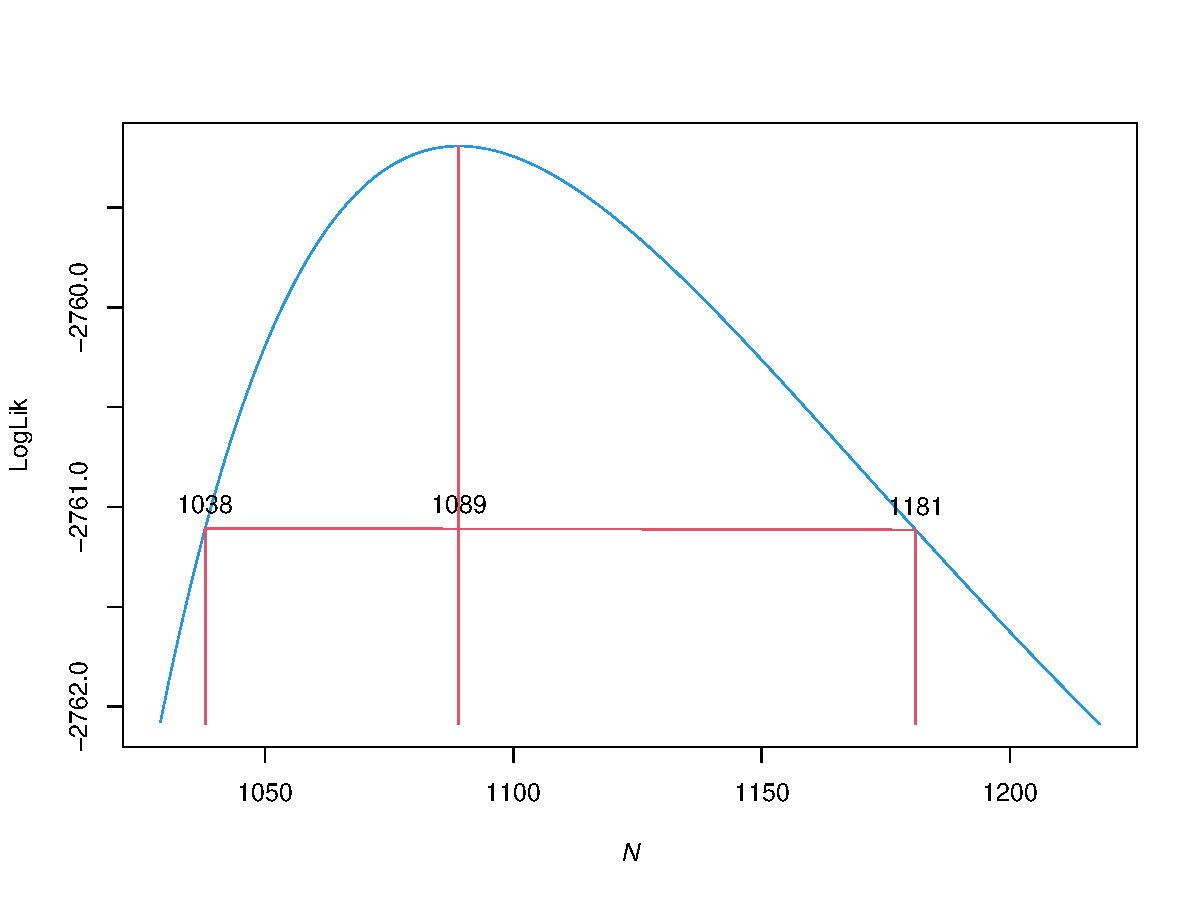
\includegraphics[width=10cm]{example_meningits_plot1.pdf}
\caption{Confidence interval for the latent class model with $k=2$ classes without covariates.}\label{fig:CI1}
\end{figure}

\subsection{Analysis with covariates}

In order to illustrate the package for the data with covariates, we consider the model selected for the same data in \cite{bartolucci2018latent} and also considered in \cite{bartolucci2024estimating}.
The model, based again on $k=2$ latent classes, follows a log-linear formulation for the conditional distribution of the capture history given the latent class, with ($i$) main effects depending on the covariate {\em Year} (centered on 2003) in a way that varies with the latent class and the specific list and ($ii$) bivariate interactions between lists (1,2) and (2,4) that do not depend on the latent class.
Moreover, the class weights are affected by the covariates {\em Age} and {\em Aez}.

The following commands are used to prepare the data, which are suitably aggregated so as to speed up the routines, and to estimate the model and build the profile confidence interval for the population size.

\begin{example*}
# build covariate matrices
Age = D[,5]
Aez = D[,6]
Year = D[,7]
W = cbind(Age,Aez)
X = Year-2003
agg = aggr_data(Y,W=W,X=X)
Wa = agg$Wa; Xa = cbind(agg$Xa); Ya = agg$Ya
colnames(Xa) = "Year"

# estimate model with covariates
biv = rbind(c(1,2),c(2,4))
est2cov = estLCCR(Ya,model ="loglin",H=2,W=Wa,X=Xa,biv=biv,free_cov="both",
                  free_biv="int",se_out=TRUE)

# estimate model without covariates and aggregated data
est2aggr = estLCCR(Ya,H=2)

# build confidence interval
CI2cov = confint(est2cov,parm=list(step=0.5))
\end{example*}
%
In this example, data aggregation is effective because there are $I=20$ distinct strata despite an overall sample size close to one thousand.
Also note that to estimate the model of interest, apart from using arguments \code{W} and \code{X}, we use argument \code{biv} that contains the list of the bivariate interactions, \code{free\_cov="both"} to require that the effect of the covariate {\em Year} on the main log-linear parameters varies with list and the latent class, and \code{free\_biv="int"} to require that the two interactions are distinct.
Finally, the model without covariates is estimated on the aggregated data in order to make a fair comparison in terms of log-likelihood and BIC.

To better understand the model structure, for the model with 2 classes it is also possible to obtain the design matrices used to parametrize the conditional distribution of the capture configurations given the covariates and the latent class as follows:

\begin{example*}
M = design_matrix_loglin(J = 4, H = 2, X = Xa, biv = biv, free_cov= "both",
                         free_biv = "int")$M
\end{example*}

\noindent obtaining an array of dimension $16\times18\times 2\time 20$, where 16 is the number of capture configurations, 18 is the number of parameters, 2 is the number of classes, and 20 is the number of strata.
Note that these design matrices are directly provided among the output arguments of the estimation function.

By the usual command \code{summary()}, applied to the previous output objects, it is possible to obtain the main estimation results; by command \code{plot(est2cov)} it is also possible to represent the profile log-likelihood function with respect to $N$, which is reported in Figure \ref{fig:CI2}.

\begin{example*}
> summary(est2cov)

Estimation of latent class models for capture-recapture data

Call:
estLCCR(Y = Ya, H = 2, model = "loglin", W = Wa, X = Xa, biv = biv,
    free_cov = "both", free_biv = "int", se_out = TRUE)

Available objects:
 [1] "beta"      "lambda"    "lk"        "N"         "np"        "AIC"
 [7] "BIC"       "M"         "tauv"      "phiv"      "Piv"       "Q"
[13] "lk1"       "lk2"       "lk3"       "lk4"       "call"      "Y"
[19] "H"         "model"     "W"         "X"         "biv"       "flag"
[25] "main"      "free_cov"  "free_biv"  "free_flag" "se_out"    "seN"
[31] "sebeta"    "selambda"

   LogLik        np       AIC       BIC
 1298.696    21.000 -2555.392 -2453.540

Population size:
      est.     s.e.
N 1358.617 164.8137

Parameters affecting the class weights:
                est.      s.e.    t-test     p-value
class2.int -3.396401 0.3559948 -9.540592 0.000000000
class2.Age  1.196301 0.4632977  2.582143 0.009818901
class2.Aez  3.881855 0.3764615 10.311426 0.000000000

Parameters affecting the conditional capture probabilities given the latent class:
                         est.       s.e.      t-test      p-value
class1.main1      -3.97671435 0.33631698 -11.8243045 0.000000e+00
class1.main2      -1.88968786 0.37771864  -5.0028981 5.647479e-07
class1.main3      -7.63620950 4.54854883  -1.6788232 9.318650e-02
class1.main4      -0.50990995 0.38807709  -1.3139398 1.888665e-01
class2.main1      -1.70265877 0.32081373  -5.3073127 1.112532e-07
class2.main2      -0.64344325 0.44667633  -1.4405134 1.497222e-01
class2.main3      -0.10490127 0.16023619  -0.6546665 5.126825e-01
class2.main4       1.27829624 0.37543619   3.4048296 6.620536e-04
class1.resp1.Year  0.47673522 0.12227804   3.8987805 9.667837e-05
class1.resp2.Year  0.09851558 0.07392841   1.3325809 1.826694e-01
class1.resp3.Year -1.38492913 2.08737446  -0.6634790 5.070238e-01
class1.resp4.Year  0.17408169 0.09860628   1.7654219 7.749288e-02
class2.resp1.Year  0.31957031 0.10915597   2.9276486 3.415358e-03
class2.resp2.Year  0.02815591 0.15996829   0.1760093 8.602866e-01
class2.resp3.Year -0.16880741 0.08695542  -1.9413098 5.222072e-02
class2.resp4.Year  0.09128870 0.17884609   0.5104316 6.097491e-01
biv1-2             2.82970526 0.29756256   9.5096146 0.000000e+00
biv2-4             1.51790409 0.36899015   4.1136710 3.894163e-05

> summary(CI2cov)

Confidence interval for the population size based on latent class models
for capture-recapture data

Call:
confint.estLCCR(object = est2cov, parm = 0.5)

Available objects:
[1] "conf"  "Nv"    "lkv"   "level" "Nh"    "lkh"   "lk1"   "lk2"   "call"

Level:
[1] 0.95

Interval limits:
[1] 1127.617 1827.117
\end{example*}

From this output, first of all we note that the BIC of the model with covariates is -2,553.5, a value much lower than that of the model without covariates, which is equal to -2,336.7.
Moreover, the estimated population size is equal to 1,359 with a 95\% confidence interval equal to (1,128, 1,827).

\begin{figure}\centering
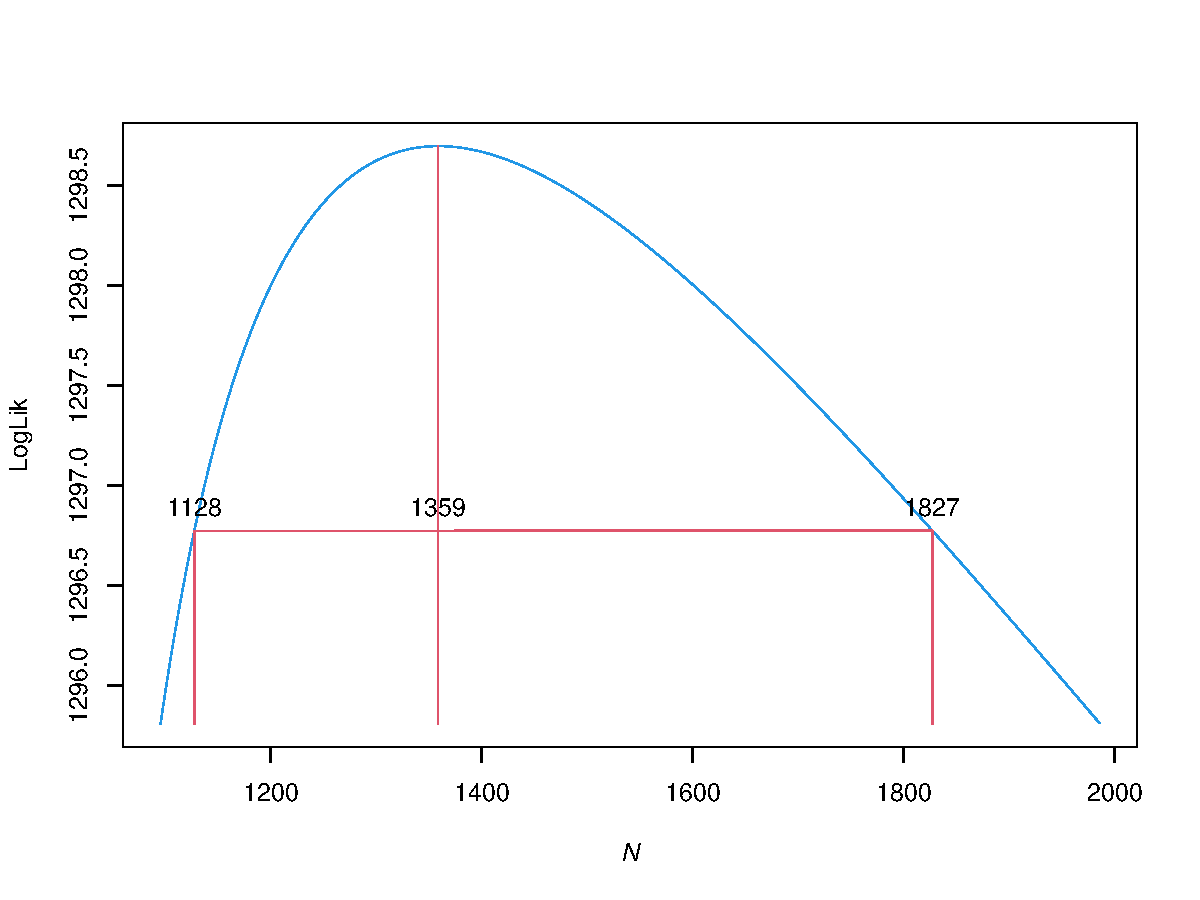
\includegraphics[width=10cm]{example_meningits_plot2.pdf}
\caption{Confidence interval for the latent class model with $k=2$ classes without covariates.}\label{fig:CI2}
\end{figure}

%It is also possible to implement a parametric bootstrap algorithm to make inference on the model parameters.
%For this aim, we can use the following commands:
%
%\begin{example*}
%# parametric bootstrap
%Nv = round(est2cov$N*est2cov$tau)
%B = 200
%NN = rep(0,B); BE = matrix(0,B,length(est2cov$be)); LA = matrix(0,B,length(est2cov$la))
%for(b in 1:B){
%  print(b)
%  sim2covb = simLCCR(2,4,est2cov$be,est2cov$la,Nv,model ="loglin",Wc=Wa,Xc=Xa,biv=biv,
%                     free_cov="both",free_biv="int")
%  est2covb = estLCCR(sim2covb$Y,model ="loglin",H=2,W=Wa,X=Xa,biv=biv,free_cov="both",
%                     free_biv="int",verb=FALSE,N0=est2cov$N,be0=est2cov$be,
%                     la0=est2cov$la)
%  NN[b] = est2covb$N; BE[b,] = est2covb$be; LA[b,] = est2covb$la
%}
%seN_boot = sd(NN); sebe_boot = apply(BE,2,sd); sela_boot = apply(LA,2,sd)
%\end{example*}
%
%The output, in terms of comparison, between asymptotic and bootstrap standard errors confirms the reliability of the first method:
%
%\begin{example*}
%> print(c(se.asym = est2cov$seN,se.boot = seN_boot))
% se.asym  se.boot
%164.8106 159.4183
%
%> print(cbind(se.asym = est2cov$sebe,se.boot = sebe_boot))
%             se.asym   se.boot
%class2.int 0.3559948 0.3817938
%class2.Age 0.4632978 0.4626715
%class2.Aez 0.3764609 0.4120886
%
%> print(cbind(la.asym = est2cov$sela,la.boot = sela_boot))
%                     la.asym     la.boot
%class1.main1      0.33631658  0.30409207
%class1.main2      0.37771766  0.37514977
%class1.main3      4.54850340 23.50245120
%class1.main4      0.38807415  0.36738809
%class2.main1      0.32081481  0.32986493
%class2.main2      0.44667931  0.44345848
%class2.main3      0.16023410  0.14503319
%class2.main4      0.37543735  0.43472499
%class1.resp1.Year 0.12227606  0.11347299
%class1.resp2.Year 0.07391988  0.06453161
%class1.resp3.Year 2.08736687 13.55333448
%class1.resp4.Year 0.09858864  0.09116597
%class2.resp1.Year 0.10915559  0.11671241
%class2.resp2.Year 0.15996830  0.17574070
%class2.resp3.Year 0.08695354  0.08996009
%class2.resp4.Year 0.17884593  0.20196567
%biv1-2            0.29756462  0.30264361
%biv2-4            0.36899302  0.36242587
%\end{example*}
%
%The estimates on the bootstrap samples can be also represented by a boxplot, using command \code{boxplot(cbind(NN,BE,LA))}, obtaining the plot in Figure \ref{fig:box-plot}.

%\section{Summary}

%This file is only a basic article template. For full details of \emph{The R Journal} style and information on how to prepare your article for submission, see the \href{https://journal.r-project.org/share/author-guide.pdf}{Instructions for Authors}.

%\section*{Acknowledgments}
%
%[RINGRAZIARE PER I DATI]

\section*{Appendix}
%
\subsection*{Score vector and information matrix}
%
The score vector and the information matrix for $\tilde{\ell}_1(\bm{\beta})$ are
\begin{eqnarray*}
\tilde{\bm{s}}_1(\bm{\beta}) &=& \sum_{i\in\mathcal{I}} \bm{W}_i'(\tilde{\bm{n}}_i-\hat{N}_i\bm\pi_i),\\
\tilde{\bm{F}}_1(\bm{\beta}) &=& \sum_{i\in\mathcal{I}} \hat{N}_i\bm{W}_i'\bm\Omega(\bm\pi_i)\bm{W}_i,
\end{eqnarray*}
where, in general, $\bm\Omega(\bm{v})=\text{diag}(\bm{v})-\bm{v}\bm{v}'$ for any probability vector $\bm{v}$.

Under the log-linear parametrization, the score vector and information matrix for $\tilde{\ell}_2(\bm{\beta})$ are
\begin{eqnarray*}
\tilde{\bm{s}}_2(\bm{\lambda}) &=& \sum_{i\in\mathcal{I}} \bm{M}_{h,i}'(\tilde{\bm{y}}_{h,i}-\tilde{n}_{h,i}\bm{q}_{h,i}),\\
\tilde{\bm{F}}_2(\bm{\lambda}) &=& \sum_{i\in\mathcal{I}} \tilde{n}_{h,i}\bm{M}_{h,i}'\bm\Omega(\bm{q}_{h,i})\bm{M}_{h,i}.
\end{eqnarray*}
Under the recursive logit parametrization, first of all note that on the basis of expression \eqref{eq:logit_matrix} we can reformulate $\tilde{\ell}_2(\bm{\beta})$ as
\[
\tilde{\ell}_2(\bm{\beta}) = \sum_{h\in\mathcal{H}}\sum_{i\in\mathcal{I}}\tilde{\bm{y}}_{h,i}'\{\bm{A}\bm{M}_{h,i}\bm{\lambda} - \bm{B}\log[\bm{1}+\exp(\bm{M}_{h,i}\bm{\lambda})]\}.
\]
Consequently, we have the following expression for the score vector and observed information matrix
\begin{eqnarray*}
\tilde{\bm{s}}_2(\bm{\beta}) &=& \sum_{h\in\mathcal{H}}\sum_{i\in\mathcal{I}} \bm{M}_{h,i}'[\bm{A}'-\text{diag}(\bm\rho_{h,i})\bm{B}']\tilde{\bm{y}}_{h,i},\\
\tilde{\bm{F}}_2(\bm{\beta}) &=& \sum_{h\in\mathcal{H}}\sum_{i\in\mathcal{I}} \bm{M}_{h,i}'\text{diag}(\bm\rho_{h,i})\text{diag}(\bm{1}-\bm\rho_{h,i})\text{diag}(\bm{B}'\tilde{\bm{y}}_{h,i})\bm{M}_{h,i},
\end{eqnarray*}
where
\[
\bm\rho_{h,i} = \text{diag}[\bm{1}+\exp(\bm{M}_{h,i}\bm{\lambda})]^{-1}\exp(\bm{M}_{h,i}\bm{\lambda}).
\]
%
\subsection*{Initialization of the EM algorithm}
%
As already mentioned, the EM algorithm can be initialized by a deterministic rule, based on the observed data, or a random rule.
These rules consist in choosing the starting values as follows:
%
\begin{itemize}
%
\item $N$ is initialized as $1.25n$ with the deterministic rule and as $u n$, where $u\sim {\rm Unif(0,1)}$, with the random rule;
%
\item with the deterministic rule, $\bm{\lambda}$ is initialized as a vector of zeros of suitable dimension when $H=1$ and by a suitable transformation of the estimates obtained under this model when $H>1$; with the random rule, the elements of the initial $\bm{\lambda}$ are drawn from a standard Normal distribution;
%
\item $\bm{\beta}$ is initialized from a vector of zeros of suitable dimension with the deterministic rule and as a vector of random numbers drawn from a standard Normal distribution with the random rule.
%
\end{itemize}

\bibliography{LCCRreferences}

\address{Francesco Bartolucci\\
  Department of Economics, University of Perugia\\
  Perugia, 06124\\
  Italy\\
  (0000-0001-7057-1421)\\
  \email{francesco.bartolucci@unipg.it}}

\address{Antonio Forcina\\
  Formerly at University of Perugia\\
  Perugia, 06124\\
  Italy\\
(0000-0001-5239-5495)\\
  \email{forcinarosara@gmail.com}}
